\documentclass[xcolor={dvipsnames}]{beamer}
%\usepackage[utf8]{inputenc}
\usetheme{Madrid}
%\usetheme{Malmoe}
\usecolortheme{beaver}
%\usecolortheme{rose}

%-------------------------------------------------------------------------------
%          -Packages nécessaires pour écrire en Français et en UTF8-
%-------------------------------------------------------------------------------
\usepackage[utf8]{inputenc}
\usepackage[frenchb]{babel}
\usepackage[T1]{fontenc}
\usepackage{lmodern}
\usepackage{textcomp}

%-------------------------------------------------------------------------------

%-------------------------------------------------------------------------------
%                          -Outils de mise en forme-
%-------------------------------------------------------------------------------
\usepackage{hyperref}
\hypersetup{pdfstartview=XYZ}
\usepackage{enumerate}
\usepackage{graphicx}
%\usepackage{multicol}
%\usepackage{tabularx}

%\usepackage{anysize} %%pour pouvoir mettre les marges qu'on veut
%\marginsize{2.5cm}{2.5cm}{2.5cm}{2.5cm}

\usepackage{indentfirst} %%pour que les premier paragraphes soient aussi indentés
\usepackage{verbatim}
%\usepackage[table]{xcolor}  
%\usepackage{multirow}
\usepackage{ulem}
%-------------------------------------------------------------------------------


%-------------------------------------------------------------------------------
%                  -Nécessaires pour écrire des mathématiques-
%-------------------------------------------------------------------------------
\usepackage{amsfonts}
\usepackage{amssymb}
\usepackage{amsmath}
\usepackage{amsthm}
\usepackage{tikz}
\usepackage{xlop}
\usepackage[output-decimal-marker={,}]{siunitx}
%-------------------------------------------------------------------------------


%-------------------------------------------------------------------------------
%                    - Mise en forme 
%-------------------------------------------------------------------------------

\newcommand{\bu}[1]{\underline{\textbf{#1}}}


\usepackage{ifthen}


\newcommand{\ifTrue}[2]{\ifthenelse{\equal{#1}{true}}{#2}{$\qquad \qquad$}}

\newcommand{\kword}[1]{\textcolor{red}{\underline{#1}}}


%-------------------------------------------------------------------------------



%-------------------------------------------------------------------------------
%                    - Racourcis d'écriture -
%-------------------------------------------------------------------------------

% Angles orientés (couples de vecteurs)
\newcommand{\aopp}[2]{(\vec{#1}, \vec{#2})} %Les deuc vecteurs sont positifs
\newcommand{\aopn}[2]{(\vec{#1}, -\vec{#2})} %Le second vecteur est négatif
\newcommand{\aonp}[2]{(-\vec{#1}, \vec{#2})} %Le premier vecteur est négatif
\newcommand{\aonn}[2]{(-\vec{#1}, -\vec{#2})} %Les deux vecteurs sont négatifs

%Ensembles mathématiques
\newcommand{\naturels}{\mathbb{N}} %Nombres naturels
\newcommand{\relatifs}{\mathbb{Z}} %Nombres relatifs
\newcommand{\rationnels}{\mathbb{Q}} %Nombres rationnels
\newcommand{\reels}{\mathbb{R}} %Nombres réels
\newcommand{\complexes}{\mathbb{C}} %Nombres complexes


%Intégration des parenthèses aux cosinus
\newcommand{\cosP}[1]{\cos\left(#1\right)}
\newcommand{\sinP}[1]{\sin\left(#1\right)}

%Fractions
\newcommand{\myfrac}[2]{{\LARGE $\frac{#1}{#2}$}}

%Vocabulaire courrant
\newcommand{\cad}{c'est-à-dire}

%Droites
\newcommand{\dte}[1]{droite $(#1)$}
\newcommand{\fig}[1]{figure $#1$}
\newcommand{\sym}{symétrique}
\newcommand{\syms}{symétriques}
\newcommand{\asym}{axe de symétrie}
\newcommand{\asyms}{axes de symétrie}
\newcommand{\seg}[1]{$[#1]$}
\newcommand{\monAngle}[1]{$\widehat{#1}$}
\newcommand{\bissec}{bissectrice}
\newcommand{\mediat}{médiatrice}
\newcommand{\ddte}[1]{$[#1)$}

%Figures
\newcommand{\para}{parallélogramme}
\newcommand{\paras}{parallélogrammes}
\newcommand{\myquad}{quadrilatère}
\newcommand{\myquads}{quadrilatères}
\newcommand{\co}{côtés opposés}
\newcommand{\diag}{diagonale}
\newcommand{\diags}{diagonales}
\newcommand{\supp}{supplémentaires}
\newcommand{\car}{carré}
\newcommand{\cars}{carrés}
\newcommand{\rect}{rectangle}
\newcommand{\rects}{rectangles}
\newcommand{\los}{losange}
\newcommand{\loss}{losanges}


%----------------------------------------------------


\usepackage{../../../../pas-math}
\usepackage{../../../../moncours_beamer}

\usepackage{amssymb,amsmath}


\newcommand{\myitem}{\item[\textbullet]}

\graphicspath{{../img/}}

\title{Séquence 4 : Géométrie du triangle}
%\author{O. FINOT}\institute{Collège S$^t$ Bernard}

%
\AtBeginSection[]
{
	\begin{frame}
		\frametitle{}
		\tableofcontents[currentsection, hideallsubsections]
	\end{frame} 

}
%
%
%\AtBeginSubsection[]
%{
%	\begin{frame}
%		\frametitle{Sommaire}
%		\tableofcontents[currentsection, currentsubsection]
%	\end{frame} 
%}

\begin{document}



\begin{frame}
  \titlepage 
\end{frame}


	
\begin{frame}
	\begin{myobj}
	\begin{itemize}
		
		\item Construire le symétrique d’un point ou d'une figure par rapport à une droite à la main où à l’aide d’un logiciel;
		\item Construire le symétrique d’un point ou d'une figure par rapport à un point, à la main où à l’aide d’un logiciel;
		\item Utiliser les propriétés de la symétrie axiale ou centrale;
		\item Identifier des symétries dans des figures.		
	\end{itemize}
\end{myobj}

\begin{mycomp}
	\begin{itemize}
		\item \kw{Chercher (Ch2)} :  s’engager    dans    une    démarche    scientifique, observer, questionner, manipuler, expérimenter (sur une feuille de papier, avec des objets, à l’aide de logiciels), émettre des hypothèses, chercher des exemples ou des contre-exemples, simplifier ou particulariser une situation, émettre une conjecture ;
		\item \kw{Raisonner (Ra3)} :  démontrer : utiliser un raisonnement logique et des règles établies (propriétés, théorèmes, formules) pour parvenir à une conclusion ;
		\item \kw{Communiquer (Co2)} :  expliquer à l’oral ou à l’écrit (sa démarche, son raisonnement, un calcul, un protocole   de   construction   géométrique, un algorithme), comprendre les explications d’un autre et argumenter dans l’échange ; 
		
	\end{itemize}
\end{mycomp}



\end{frame}

\section{Inégalité triangulaire}


\begin{frame}
	\begin{myprop}
		
		\begin{itemize}
			\item Dans un triangle la longueur d'un coté est \kword{inférieure à la somme} des longueurs des deux autres côtés.\pause
			
			\item  Si la longueur du plus grand coté est égale à la somme des deux autres, le triangle est \kword{plat}.
		\end{itemize}
			
			

		
	\end{myprop}
	
	\begin{block}{Méthode}
		Pour vérifier qu'un \kword{triangle est constructible}, \pause on vérifie que la longueur du plus grand côté  est inférieure à la somme des deux autres.
	\end{block}
\end{frame}


\begin{frame}
	\begin{myexs}
		
		\begin{itemize}
			\item Dans le triangle ABC ci-contre on a $AB < AC + CB.$
				\begin{center}
					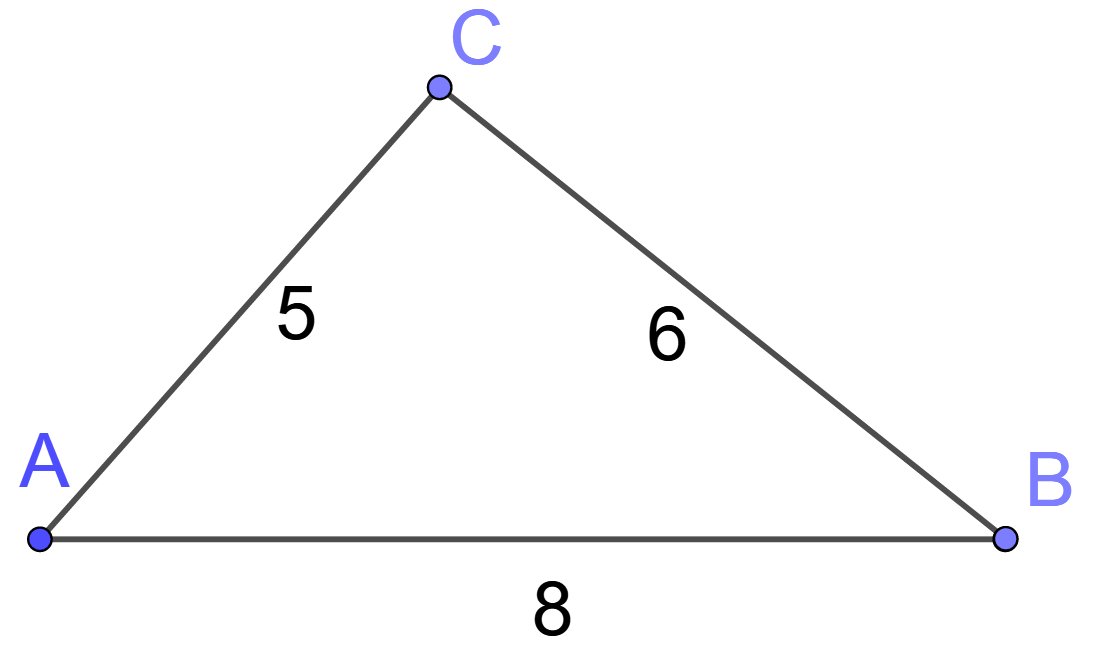
\includegraphics[scale=0.25]{triangle1}\pause
					
					%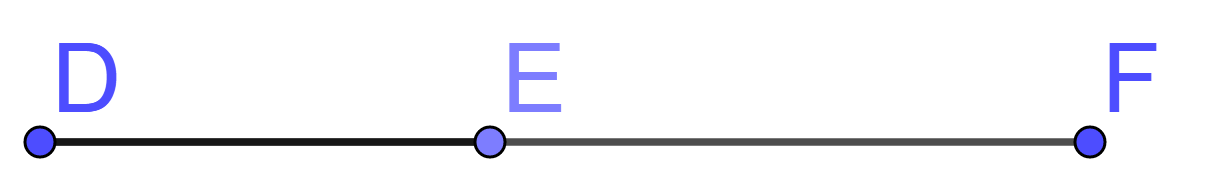
\includegraphics[scale=0.2]{triangle2}
				\end{center}
			
			\item 	Un triangle de cotés 8 cm, 5 cm et 6 cm est constructible (8 < 11).
		\end{itemize}
		
		
		
	\end{myexs}
\end{frame}

\begin{frame}
	\begin{myexs}
		
		\begin{itemize}
			\item Le triangle $DEF$, tel que $DE = 7$ cm, $DF = 3$ cm et $FE = 4$ cm est plat, les points sont alignés ($4 + 3 = 7$).
			\begin{center}
				%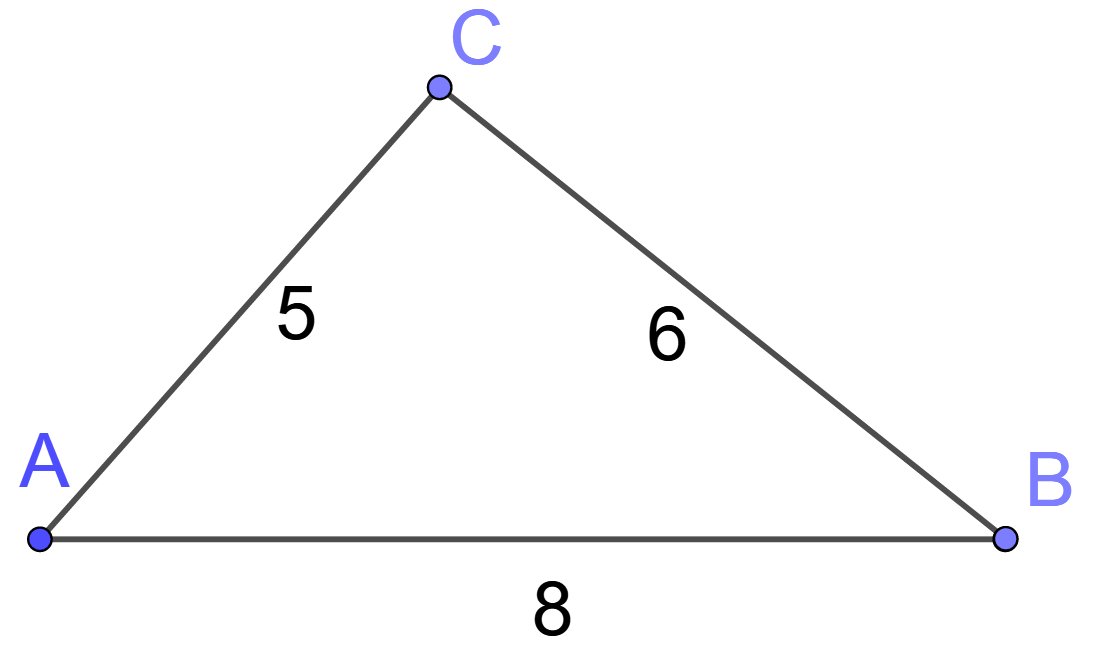
\includegraphics[scale=0.25]{triangle1}\pause
				
				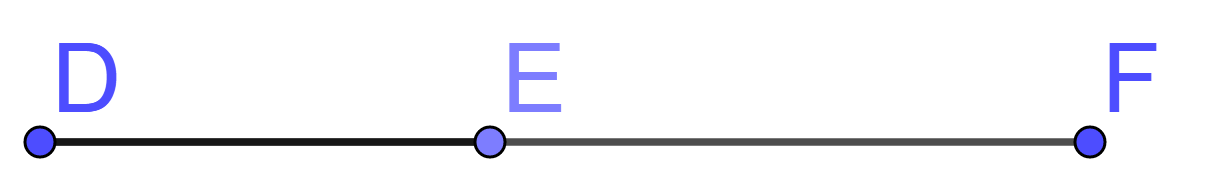
\includegraphics[scale=0.2]{triangle2}\pause
			\end{center}
			
			\item 	Un triangle de coté 10 cm, 4 cm et 5 cm n'est pas constructible ($10 > 4 + 5$).
		\end{itemize}
		
		
		
	\end{myexs}
\end{frame}

\section{Droites remarquables}

\section{Angles d'un triangle}

\begin{frame}
	\begin{myprop}
		La \kword{somme des mesures} des angles d'un triangle vaut 180\degree.\pause
	\end{myprop}


	\begin{myex}
		\begin{center}
			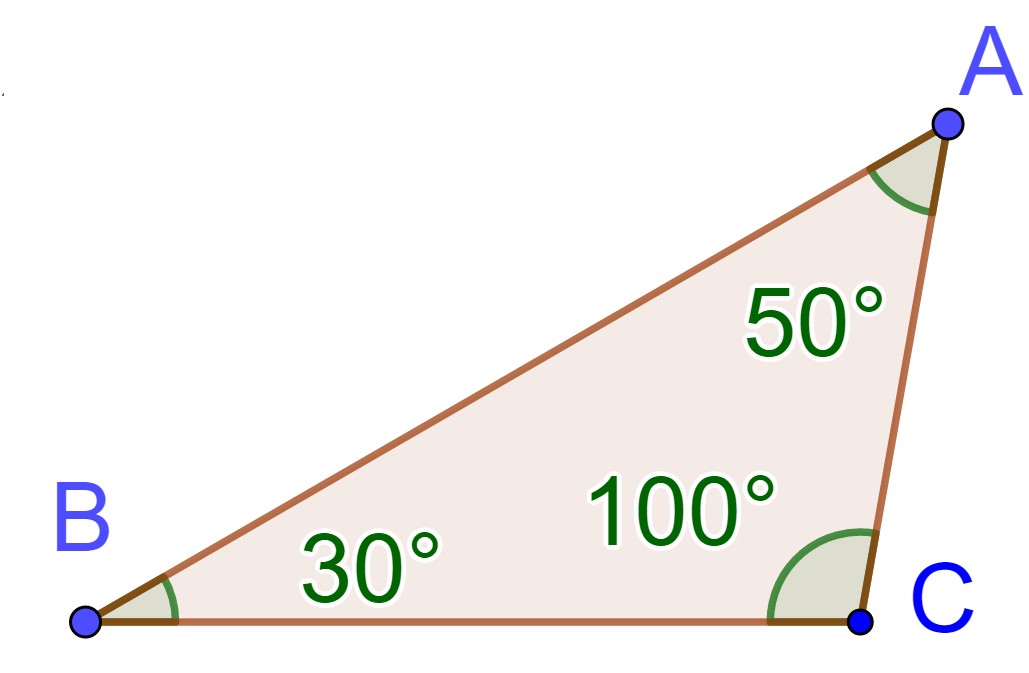
\includegraphics[scale=0.22]{quelconque}\pause
		\end{center}
	
		Dans le triangle $ABC$, on a \pause $\hat{A} + \hat{B} + \hat{C} = 180\degree$
	\end{myex}
\end{frame}

\begin{frame}
	\begin{myex}
		\begin{center}
			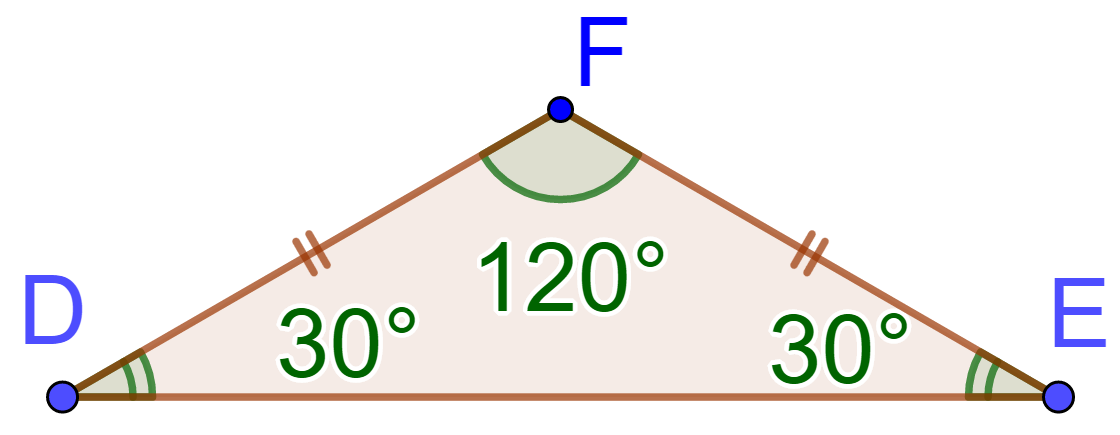
\includegraphics[scale=0.22]{isocele}\pause
		\end{center}
		
		Dans un triangle isocèle, \pause les deux angles à la base sont égaux (ici 30\degree).
	\end{myex}
\end{frame}


\begin{frame}
	\begin{myex}
		\begin{center}
			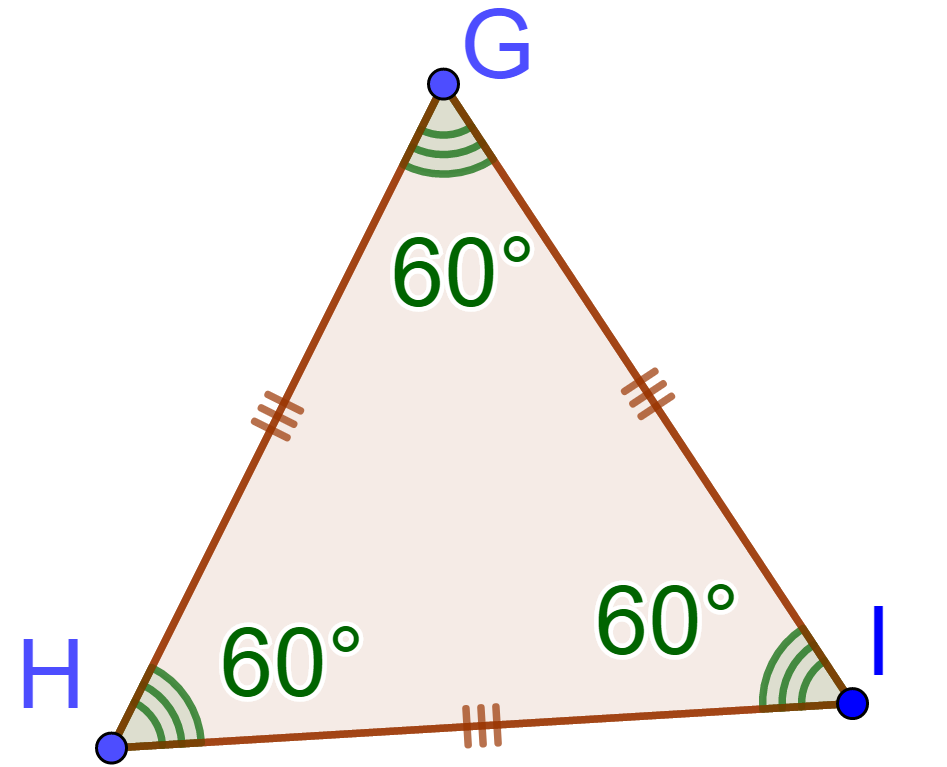
\includegraphics[scale=0.22]{equilateral}\pause
		\end{center}
		
			Dans un triangle équilatéral, \pause tous les angles sont égaux et mesurent 60\degree.
	\end{myex}
\end{frame}

\begin{frame}
	\begin{myex}
		\begin{center}
			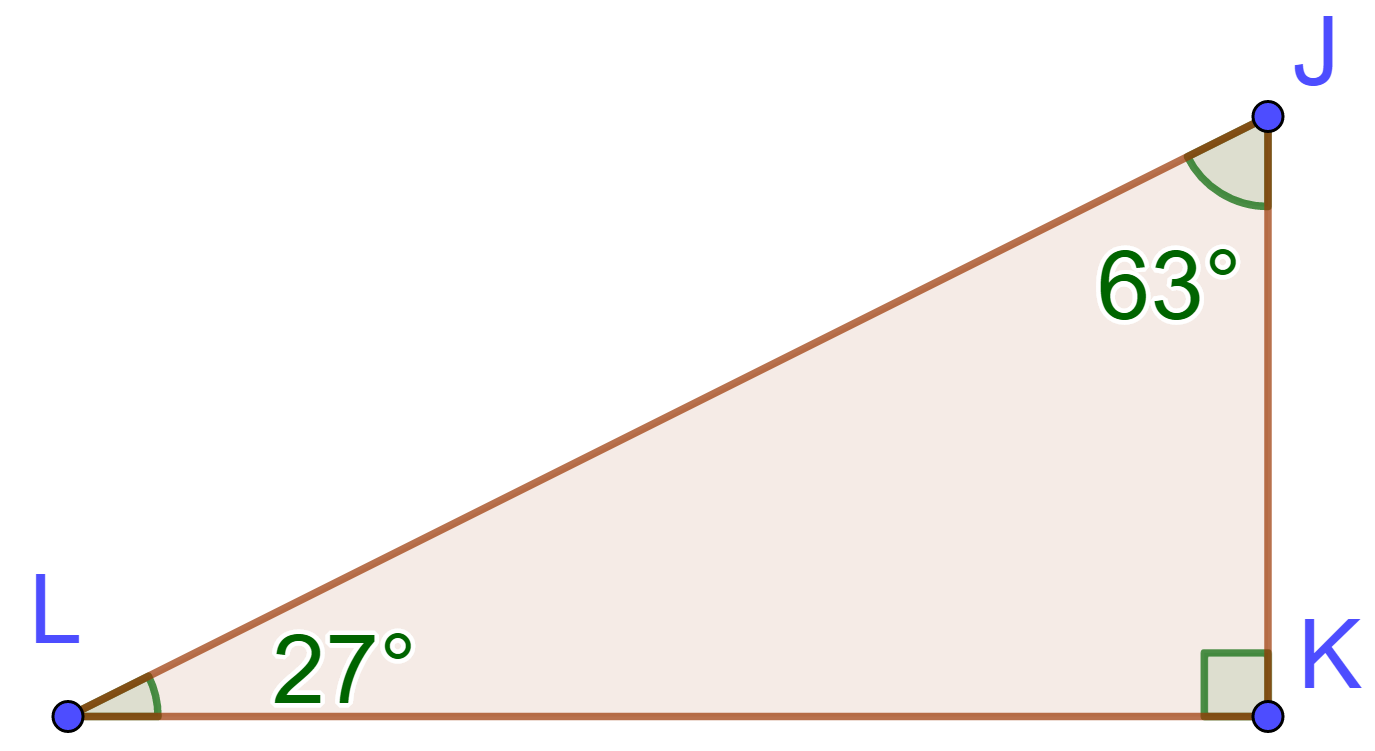
\includegraphics[scale=0.22]{rectangle}\pause
		\end{center}
		
		Dans un triangle rectangle, \pause la somme des mesures des angles non droits vaut 90\degree.
	\end{myex}
\end{frame}
\end{document}